\documentclass[../../../../main.tex]{subfiles}

\begin{document}

\section*{第1問}

\begin{proof}[解]
\[
(x^3+ax^2+bx+c)^2=(x^2-1)(x^2+px+q)^2+D
\]
が $x$ についての恒等式である。左辺，右辺を各々 $f(x),g(x)$ とする。
\[
f(x)=x^6+2ax^5+(2b+a^2)x^4+(2c+2ab)x^3+(2ac+b^2)x^2+2bcx+c^2
\]
\[
g(x)=x^6+2px^5+(p^2+2q-1)x^4+(2pq-2p)x^3+(q^2-p^2-2q)x^2-2pqx-q^2+D
\]
係数比較して，
\[
a=p, \quad 2b=2q-1, \quad ab+c=pq-p, \quad 2ac+b^2=q^2-p^2-2q, \quad bc=-pq, \quad c^2=-q^2+D
\]
を得る。したがって，第1，2式から
\[
a=p, \qquad b=q-\frac12 \quad \cdots \text{①}
\]
第3式に代入して
\[
c=-\frac12 p \quad \cdots \text{②}
\]
第4式から $q=-\dfrac14$ となり①より $b=-\dfrac34$ となる。第5式から，
\[
bc=-pq \quad\Longrightarrow\quad \frac38p=\frac14p \quad\therefore\ p=0
\]
だから，①②より $a=c=0$ で，最後の式から，
\[
D=c^2+q^2=0+\frac{1}{16}=\frac{1}{16}
\]
\end{proof}

\newpage

\section*{第2問}

\begin{proof}[解]
$A=(bc-1)(ca-1)(ab-1)$ とおく。以下 $a,b,c\in\mathbb{N}$ に注意する。
\[
A=(abc)^2-(a^2bc+ab^2c+abc^2)+(bc+ca+ab)-1 = (abc)^2-(a+b+c)(abc)+(bc+ca+ab-1)
\]
だから，$A/abc\in\mathbb{Z}$ となる時（$bc+ca+ab-1$）$/abc\in\mathbb{Z}$ つまり $bc+ca+ab-1$ が $abc$ で割り切れる。（以上(1)）

したがって，$k\in\mathbb{N}$ に対し（$\because bc+ca+ab-1>0$）
\[
\frac{bc+ca+ab-1}{abc}=k \iff \frac1a+\frac1b+\frac1c-\frac{1}{abc}=k \quad \cdots \text{①}
\]
とおける。又，$a\in\mathbb{N}$ 及び題意から
\[
2\le a<b<c, \quad a,b,c\in\mathbb{N} \quad \cdots \text{②}
\]
である。②から
\[
\frac1a+\frac1b+\frac1c-\frac1{abc}<\frac1a+\frac1a+\frac1a-\frac1{abc}=\frac1a\left(3-\frac1{bc}\right)
\]
となり，①及び $k\in\mathbb{N}$ から
\[
1<\frac1a\left(3-\frac1{bc}\right) \quad\therefore\ a<3-\frac1{bc}<3 \quad (\because a,b,c>0)
\]
②とあわせて $a=2$ が必要。①に代入して
\[
\frac1b+\frac1c-\frac12\cdot\frac1{bc}=k-\frac12 \quad \cdots \text{②}'
\]
同様にして，
\[
\frac12\le k-\frac12<\frac1b\left(2-\frac{1}{2c}\right) \quad\therefore\ b<2\left(2-\frac{1}{2c}\right)<4 \quad (\because b,c>0)
\]
だから②より，$b=3$ が必要。②'に代入して
\[
\frac1c-\frac13\cdot\frac1c=k-\frac12-\frac13 \quad\therefore\ c=\frac{1}{\frac65k-1} \quad \left(\because k\in\mathbb{N}\text{から}\frac65k-1>0\right)
\]
$c\in\mathbb{N}$ から $c>b=3$ より
\[
\frac{1}{\frac65k-1}>3 \iff k<\frac{25}{18} \quad \left(\because\frac65k-1>0\right)
\]
から，$k=1$ が必要で，この時 $c=5$ で条件をみたし十分。

題意をみたす $a,b,c$ の組は，①，②をみたす $k$ が存在する $(a,b,c)$ の組と同じだから以上より，
\[
(a,b,c)=(2,3,5)
\]
\end{proof}

\newpage

\section*{第3問}

\begin{proof}[解]
\begin{enumerate}
  \item[(1)] $L$ の方程式は $\dfrac{r}{\sqrt2}x+\dfrac{r}{\sqrt2}y=r^2$ $\therefore x+y=\sqrt2r$ だから，方向ベクトル $\vec v=\begin{pmatrix}1\\-1\end{pmatrix}$ で，$P$ が $L$ 上の点の時，$a+b=\sqrt2r$ で，これは $P'(b,a)$ が $L$ 上にあることも意味する。したがって，$t$ を実数として
  \[
  \begin{pmatrix}c\\d\end{pmatrix}=\begin{pmatrix}b\\a\end{pmatrix}+(a-b)t\begin{pmatrix}1\\-1\end{pmatrix}
  \]
  と表せる。（$\because P\ne\left(\dfrac{r}{\sqrt2},\dfrac{r}{\sqrt2}\right)$ より，$a\ne b$）したがって，
  \[
  \begin{cases}
  c=b+(a-b)t=at+(1-t)b \\
  d=a+(a-b)t(-1)=(1-t)a+tb
  \end{cases}
  \]
  と表せる。

  \begin{center}
  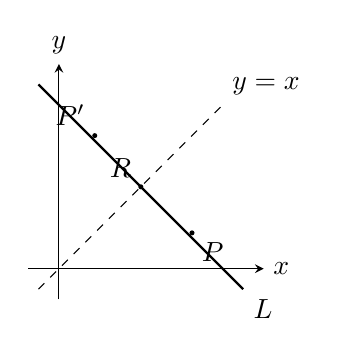
\begin{tikzpicture}[scale=1.3, >=stealth]
    \draw[->] (-0.3,0) -- (2,0) node[right] {$x$};
    \draw[->] (0,-0.3) -- (0,2) node[above] {$y$};
    \draw[thick] (-0.2,1.8) -- (1.8,-0.2) node[below right] {$L$};
    \draw[dashed] (-0.2,-0.2) -- (1.6,1.6) node[above right] {$y=x$};
    \fill (0.8,0.8) circle (0.7pt) node[above left] {$R$};
    \fill (1.3,0.35) circle (0.7pt) node[below right] {$P$};
    \fill (0.35,1.3) circle (0.7pt) node[above left] {$P'$};
  \end{tikzpicture}
  \end{center}

  \item[(2)] $\begin{pmatrix}c\\d\end{pmatrix}=t\begin{pmatrix}a\\b\end{pmatrix}+(1-t)\begin{pmatrix}b\\a\end{pmatrix}$ より，$(c,d)$ は $\overline{PP'}$ 上にある時，$P'P$ の $t:1-t$ 内分点である。これと接点 $R$ が $\overline{PP'}$ の中点であることから，$t$ の条件は
  \[
  \frac12\le t\le1
  \]
\end{enumerate}
\end{proof}

\newpage

\section*{第4問}

\begin{proof}[解]
題意から，
\[
\begin{cases}
a_1=1 \\
a_n+a_{n+1}=-3n \\
a_na_{n+1}=C_n
\end{cases}
\]
である。したがって，
\[
a_{n+1}+\frac32(n+1)-\frac34=-\left\{a_n+\frac32n-\frac34\right\}
\]
だから，くり返し用いて，
\[
a_n=(-1)^{n-1}\left\{1+\frac32-\frac34\right\}-\frac32n+\frac34 = \frac74(-1)^{n-1}+\frac34-\frac32n
\]
\[
\therefore\
\begin{cases}
a_{2k}=-3k-1 \\
a_{2k-1}=-3k+4
\end{cases}
\]
となるので，
\[
\begin{cases}
C_{2k-1}=a_{2k-1}\cdot a_{2k}=(-3k+4)(-3k-1) \\
C_{2k}=a_{2k}\cdot a_{2k+1}=(-3k-1)(-3k-1+3)
\end{cases}
\quad \cdots \text{②}
\]
より，
\[
\sum_{k=1}^{2p}C_k=\sum_{k=1}^{p}(C_{2k-1}+C_{2k}) = \sum_{k=1}^{p}(-3k-1)(-6k+5) \quad (\because②) = \sum_{k=1}^{p}(18k^2-9k-5)
\]
\[
=18\cdot\frac16 p(p+1)(2p+1)-\frac92p(p+1)-5p = 3p(p+1)(2p+1)-\frac92p(p+1)-5p
\]
\[
=p(p+1)\left\{6p+3-\frac92\right\}-5p = 6p^3+\frac92p^2-\frac{13}{2}p
\]
\end{proof}

\newpage

\section*{第5問}

\begin{proof}[解]
$h(x)=f(x)-g(x)$ とおく。$h(x)$ は4次のモニック多項式であり，$h(1)=h(-1)=0$ より，因数定理から，$\alpha,\beta\in\mathbb{R}$ として
\[
h(x)=(x+1)(x-1)(x^2+\alpha x+\beta) \quad \cdots \text{①}
\]
とかける。したがって，
\[
\{h(x)\}^2=(x^2-1)^2(x^4+2\alpha x^3+(\alpha^2+2\beta)x^2+2\alpha\beta x+\beta^2)
\]
だから，$A=\displaystyle\int_{-1}^1\{h(x)\}^2dx$ として，
\[
A=2\int_0^1(x^2-1)^2(x^4+(\alpha^2+2\beta)x^2+\beta^2)dx
\]
\[
\therefore\ \frac12A=\alpha^2\int_0^1(x^2-1)^2x^2dx+2\beta\int_0^1(x^2-1)^2x^2dx+\beta^2\int_0^1(x^2-1)^2dx+\int_0^1x^4(x^2-1)^2dx
\]
\[
=\alpha^2\int_0^1(x^2-1)^2x^2dx+\frac{8}{15}\beta^2+\frac{16}{105}\beta+\int_0^1x^4(x^2-1)^2dx
\]
\[
=\alpha^2\int_0^1(x^2-1)^2x^2dx+\frac{8}{15}\left\{\left(\beta+\frac17\right)^2-\frac{1}{49}\right\}+\int_0^1x^4(x^2-1)^2dx \quad \cdots \text{②}
\]
である。$\displaystyle\int_0^1x^2(x^2-1)^2dx>0$ だから，②より，$A$ の $\min$ を与える $(\alpha,\beta)$ は，$(\alpha,\beta)=\left(0,-\dfrac17\right)$ である。 $\cdots$③ さて，①から，③の時，
\[
h(x)=x^4+\alpha x^3+(\beta-1)x^2-\alpha x-\beta = x^4-\frac{8}{7}x^2+\frac17
\]
だから，$(a,b,c,d)=\left(0,\dfrac{8}{7},-1,-\dfrac17\right)$ とおけば良い。
\end{proof}

\newpage

\section*{第6問}

\begin{proof}[解]
$-1\le a\le1$ から，
\[
I(a)=\int_{-1}^a(a-x)\cdot e^xdx+\int_a^1(x-a)e^xdx
\]
\[
=a\int_{-1}^ae^xdx-\int_{-1}^axe^xdx-a\int_a^1e^xdx+\int_a^1xe^xdx
\]
とする。
\[
I'(a)=\int_{-1}^ae^xdx+ae^a-\int_a^1e^xdx+ae^a-ae^a-ae^a = \int_{-1}^ae^xdx-\int_a^1e^xdx
\]
\[
=\left[e^x\right]_{-1}^a-\left[e^x\right]_a^1=\left(e^a-\frac1e\right)-(e-e^a)=2e^a-\left(e+\frac1e\right)
\]
から，下表を得る（$I'(a)=0\iff e^a=\dfrac{e+1/e}{2}=\dfrac{e^2+1}{2e}$，つまり $a=\log\dfrac{e^2+1}{2e}$）

\begin{center}
\begin{tabular}{c|c|c|c|c|c}
$a$ & $-1$ & & $\log\dfrac{e^2+1}{2e}$ & & $1$ \\
\hline
$I'$ & & $-$ & $0$ & $+$ & \\
\hline
$I$ & & $\searrow$ & & $\nearrow$ &
\end{tabular}
\end{center}

したがって，最大値は $I(1), I(-1)$ のうち小さくない方である。
\[
I(1)=\int_{-1}^1(1-x)e^xdx=\left[e^x(2-x)\right]_{-1}^1=e-\frac3e
\]
\[
I(-1)=\int_{-1}^1(x+1)e^xdx=\left[e^x\cdot x\right]_{-1}^1=e+\frac1e
\]
一方，$I(-1)>I(1)$（$\because e>0$）だから，もとめる $\max$ は
\[
I(-1)=e+\frac1e
\]
\end{proof}

\end{document}
